\documentclass[mat1]{fmfdelo}
% \documentclass[fin1]{fmfdelo}
% \documentclass[isrm1]{fmfdelo}
% \documentclass[mat2]{fmfdelo}
% \documentclass[fin2]{fmfdelo}
% \documentclass[isrm2]{fmfdelo}

% aktivirajte pakete, ki jih potrebujete
% \usepackage{tikz}
\usepackage{graphicx}

% za številske množice uporabite naslednje simbole
\newcommand{\R}{\mathbb R}
\newcommand{\N}{\mathbb N}
\newcommand{\Z}{\mathbb Z}
\newcommand{\C}{\mathbb C}
\newcommand{\Q}{\mathbb Q}

% matematične operatorje deklarirajte kot take, da jih bo Latex pravilno stavil
% \DeclareMathOperator{\conv}{conv}

% na razpolago so naslednja matematična okolja, ki jih kličemo s parom 
% \begin{imeokolja}[morebitni komentar v oklepaju] ... \end{imeokolja}
%
% definicija, opomba, primer, zgled, lema, trditev, izrek, posledica, dokaz
% 


% vstavite svoje definicije ...
%  \newcommand{}{}


% naslednje ukaze ustrezno napolnite
\avtor{Živa Urbančič} 

\naslov{Grupa kit in njene upodobitve}
\title{Braid group and her representations}

% navedite ime mentorja s polnim nazivom: doc.~dr.~Ime Priimek, 
% izr.~prof.~dr.~Ime Priimek, prof.~dr.~Ime Priimek
% uporabite le tisti ukaz/ukaze, ki je/so za vas ustrezni 
\mentor{izr. prof. dr. Sašo Strle}
% \mentorica{}
% \somentor{}
% \somentorica{}
% \mentorja{}{}
% \mentorici{}{}

\letnica{2016} % leto diplome

%  V povzetku na kratko opišite vsebinske rezultate dela. Sem ne sodi razlaga organizacije dela --
%  v katerem poglavju/razdelku je kaj, pač pa le opis vsebine.
\povzetek{}

%  Prevod slovenskega povzetka v angleščino. 
\abstract{}

% navedite vsaj eno klasifikacijsko oznako --
% dostopne so na www.ams.org/mathscinet/msc/msc2010.html
\klasifikacija{}
\kljucnebesede{} % navedite nekaj ključnih pojmov, ki nastopajo v delu
\keywords{} % angleški prevod ključnih besed


\begin{document}

\section{Uvod}

Teorija kit je močno povezana s teorijo vozlov, a je zanimiva in pomembna tudi kot samostojna raziskovalna smer. Kite je prvi definiral avstrijski matematik Emil Artin v svojem članku \emph{"Theorie der Z\''{o}pfe"}, ki je bil objavljen leta $1925$. Glavni izrek članka reši problem klasifikacije kit, a z njegovim dokazom ni bil zadovoljen. Opisal ga je kot "neprepričljivega" in ga nato v članku iz leta 1947 z naslovom \emph{"Theory of braids"} zapisal na način, ki prepriča tudi najbolj rigorozne in skeptične bralce. Tako je teorijo pravzaprav postavil na njene temelje. Leta raziskovanja so prinesla tudi nekatere ekvivalentne definicije, ki so jih matematiki prilagodili potrebam preučevanja in uporabe v drugih matematičnih smereh. Uporablja se recimo v mehaniki fluidov, statistični mehaniki, nekomutativni kriptografiji in pri reševanju polinomskih enačb.???

\section{Prosta grupa in upodobitve}

To poglavje je namenjeno razlagi algebraične teorije, ki jo bomo potrebovali za nadaljne raziskovanje. Vpeljali bomo pojme, ki jih potrebujemo, da lahko definiramo, kaj je upodobitev in jo kasneje tudi poiščemo.\\
Naj bo $X = \{ x_1,\ x_2,\ \ldots,\ x_n \}$ neka množica (lahko je tudi neskončna). Imenujmo jo \emph{abeceda}, posamezen element pa imenujmo \emph{črka}. Definirajmo množico $S$ kot množico vseh besed, ki jih lahko sestavimo iz črk abecede $X$.

\begin{trditev}
Množica $S$ je za operacijo stikanja besed ($x \circ y = xy, \ x, y \in X$) polgrupa.
\end{trditev}

\begin{dokaz}
Operacija je očitno asociativna.
\end{dokaz}

\begin{opomba}
Polgrupo $(S, \circ)$ imenujemo \emph{prosta polgrupa}.
\end{opomba}

\begin{opomba}
Če množici $S$ dodamo še prazno besedo, postane za operacijo stikanja monoid.
\end{opomba}

Vprašanje, kaj $S$ (z dodano prazno besedo) manjka do grupe, nas motivira k definiciji množice $X^{-1} = \{x_1^{-1},\ x_2^{-1}, \ \ldots, \ x_n^{-1}\}$. Nova abeceda naj bo $A = X \cup X^{-1}$. Množica besed nad $A$ pa še ni, kar iščemo, saj v besedah ne želimo podbesed oblike $x_ix_i^{-1}$.

\begin{definicija}
Beseda nad $A$ je \emph{reducirana}, če ne vsebuje podbesede oblike $xx^{-1}$ ali $x^{-1}x$, kjer je $x\in A$.
\end{definicija}

Označimo z $F_x$ množico vseh reduciranih besed nad $A$. Na njej definirajmo operacijo $\circ$, ki stakne besedi in ju zapiše v reducirani obliki (tj. pokrajša neželene podbesede).



\section{Grupa kit}

\subsection{Definicija grupe kit}

Kot je bilo omenjeno v uvodu, lahko grupo kit definiramo na različne (ekvivalentne) načine, kakor najbolj ustreza našemu raziskovanju. V tem razdelku bomo podali (algebraično in) geometrijsko definicijo kite (nekatere druge bralec lahko najde v [?] in [?]) in se prepričali, da množica kit, če na njej definiramo operacijo stikanja, res postane grupa. Pri tem bomo morali obravnavati tudi, kdaj sta kiti ekvivalentni, pri čemer bomo sledili [?] in [?].\\
Kite si lahko zelo lahko predstavljamo kot skupek pramenov, ki so prepleteni med seboj. To je zgolj opis, za podrobnejše preučevanje potrebujemo bolj formalno in matematično korektno razlago. To nas napelje k zapisu geometrijske definicije kite.\\
Imejmo premici $\{y = z = 0\}$ ter $\{y = 0, z = 1\}$ v $\R^3$. Na vsaki izmed premic izberemo $m$ točk z abscisami $x=1,\ 2,\ \ldots,\ m$.

\begin{definicija}
\emph{Kita z m prameni} je množica $m$ disjunktnih gladkih poti, ki povezujejo točke s prve izbrane premice s tistimi z druge (v poljubnem vrstnem redu). Projekcija posamezne poti na ravnino $z$ mora biti difeomorfizem - imenujemo ga \emph{pramen} kite.
\end{definicija}

\begin{figure}[h!]
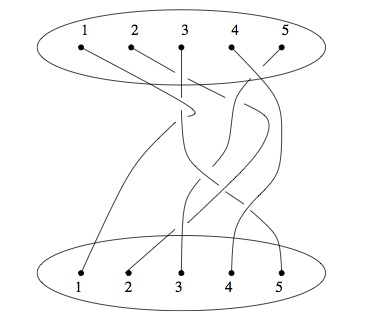
\includegraphics[height = 5cm]{Primer_kite_1}
\caption{Primer kite s 5 prameni.}
\end{figure}

%\begin{definicija}
%Kiti $B_0$ in $B_1$ sta \emph{ekvivalentni}, če sta si izotopni.
%\end{definicija}





\section*{Slovar strokovnih izrazov}

\geslo{Živa}{Najboljša v vsem ever.}
\geslo{}{}


% seznam uporabljene literature
\begin{thebibliography}{99}

%\bibitem{}

\end{thebibliography}

\end{document}

